% !TeX root = thesis.tex
%--------------------------------------------------------------------%
%
% Template TA LaTeX Teknik Informatika ITERA.
% Editor: Radhinka Bagaskara, Martin C.T. Manullang, iwawiwi
% Version 2024.1
%
% Berdasarkan "Templat LaTeX Tesis Informatika ITB" oleh Petra Barus & Peb Ruswono Aryan
% https://github.com/petrabarus/if-itb-latex
%--------------------------------------------------------------------%
%
% Berkas ini berisi struktur utama dokumen LaTeX yang akan dibuat.
%
%--------------------------------------------------------------------%

% Set jenis dokumen Tugas Akhir
\documentclass[12pt, a4paper, onecolumn, oneside, final]{report}
% \documentclass[11pt, a5paper, onecolumn, final]{report} % Untuk versi perpustakaan

%-------------------------------------------------------------------%
%
% Konfigurasi dokumen LaTeX untuk laporan tesis IF ITB
% 
%
% @author Radhinka Bagaskara, Petra Novandi (ITB)
%
%-------------------------------------------------------------------%
%
% Berkas asli berasal dari Steven Lolong
%
%-------------------------------------------------------------------%

% Import package penting
\usepackage[utf8]{inputenc}
\usepackage{subcaption} % Paket untuk mengatur gambar berdampingan
\usepackage{graphicx}
\usepackage{titling}
\usepackage{blindtext} % Untuk lorem ipsum
\usepackage{sectsty} % Untuk header & judul
\usepackage{chngcntr} % Untuk penambahan nomor caption
\usepackage{etoolbox} % Untuk CRUD variabel (?)
\usepackage{array} % % Untuk tabel di math mode
\usepackage{float} % Untuk tabular
\usepackage{longtable} % Untuk tabel yang potong halaman
\usepackage{amsmath} % Untuk equation
\usepackage{enumitem} % Untuk list enumerate yg lebih rapi
\usepackage[bookmarks]{hyperref}
\usepackage{lipsum}
\hypersetup{
	colorlinks,
	citecolor=black,
	filecolor=black,
	linkcolor=black,
	urlcolor=black
}

% Ukuran kertas A4
\special{papersize=215mm,297mm}

% Setting margin
\usepackage[top=3cm,bottom=3cm,left=4cm,right=3cm]{geometry}

% Setting indensasi
\usepackage{indentfirst}
\usepackage{parskip}
\setlength{\parindent}{20pt}
\setlength{\parskip}{0pt}

% Linespacing 1.5. Tidak serupa dengan 1.5 di Word (RDB)
\renewcommand{\baselinestretch}{1.5}

% Agar tidak ada kata yang terpotong setiap baris kalimat
\hyphenpenalty=10000

% Font
%\usepackage{mathptmx} 
\usepackage{newtx} 
% Times New Roman itu copyright dari Microsoft. Ini alternatifnya (RDB)

% Judul bahasa Indonesia
\usepackage[bahasa]{babel}

% Format tanggal
\usepackage[style=ddmmyyyy,datesep=-]{datetime2}



% Format citation
\usepackage[backend=biber,citestyle=ieee]{biblatex}

% Remove "In:" before journal titles
\renewbibmacro{in:}{}

% Ensure URLs, DOIs, and ISSNs use the default font (e.g., Times New Roman)
\renewcommand*{\UrlFont}{\rmfamily} % Use default font for URLs
\DeclareFieldFormat{issn}{#1}       % Use default font for ISSN
\DeclareFieldFormat{doi}{#1}        % Use default font for DOI

% Remove DOI and URL fields if not needed (optional)
\AtEveryBibitem{
  \clearfield{doi}
  \clearfield{url}
}

\DeclareLanguageMapping{bahasa}{english}



% Package untuk link di daftar isi.
\usepackage{titlesec}       % Package Format judul
\usepackage{parskip}
\usepackage{ragged2e}		% Alignment
\usepackage{multirow}		% Untuk bisa merge cell di tabel
\usepackage{tikz}			% Untuk menggambar kotak pas foto
\usepackage{setspace}		% Spacing paragraph
\usepackage{fancyhdr}		% Agar nomor halaman di pojok kanan atas
\usepackage{caption} 		% Caption gambar & tabel
\usepackage{comment}

\captionsetup[figure]{font=footnotesize} % Mengatur caption gambar ke 10pt (footnotesize)
\captionsetup[figure]{labelsep=space} % Mengubah ":" menjadi spasi setelah nomor gambar
\captionsetup[table]{font=footnotesize}
\captionsetup[table]{labelsep=space}
\captionsetup[equation]{font=footnotesize}
\captionsetup[lstlisting]{font=footnotesize, labelsep=space}

% Setting supaya nomor halaman pertama dengan "chapter"
% berada di kanan atas
\fancypagestyle{plain}{%
	\fancyhf{}%
	\renewcommand{\headrulewidth}{0pt}
	\fancyhead[R]{\thepage}
}

% Setting judul
\chapterfont{\centering \large}
\titleformat{\chapter}[display]%
  	{\large\centering\bfseries}%
  	{\chaptertitlename\ \thechapter}{0pt}%
  	{\large\bfseries\uppercase}
\titleformat{\section}%
	{\normalfont\normalsize\bfseries}{\thesection}{1em}{}
\titleformat{\subsection}%
	{\normalfont\normalsize\bfseries}{\thesubsection}{1em}{}

%\makeatletter
%\def\@makechapterhead#1{%
%  \vspace*{-2cm} % GESER KE ATAS (coba-coba sampai pas di margin)
%  {\parindent \z@ \centering
%   \normalfont
%   \interlinepenalty\@M
%   \Large\bfseries \MakeUppercase{\@chapapp\space \thechapter}\par\nobreak
%   \vskip 0pt
%   \Large\bfseries \MakeUppercase{#1}\par\nobreak
%   \vskip 20pt
%  }}
%\makeatother

    
% Setting spacing di setiap judul chapter
\titlespacing*{\chapter}{0pt}{0pt}{30pt}
\titlespacing*{\section}{0pt}{20pt}{0pt}
\titlespacing*{\subsection}{0pt}{20pt}{0pt}
\titlespacing*{\subsubsection}{0pt}{20pt}{0pt}

\usepackage{listings}
\usepackage{xcolor}
\usepackage{geometry}


% Setting nomor pada subbsubsubbab
\setcounter{secnumdepth}{3}

% Counter untuk figure dan table, agar bertambah walaupun lintas subbab
\counterwithout{figure}{section}
\counterwithout{table}{section}

% Supaya tidak ada garis di header
\renewcommand{\headrulewidth}{0pt}

% Setting daftar isi, daftar gambar, daftar tabel, daftar rumus
\usepackage[titles]{tocloft}
\setlength{\cftbeforechapskip}{5.2pt}
% ------------------------------------------------------------------
% Make the vertical gap before *every* figure/table entry the same:
\setlength{\cftbeforefigskip}{0pt}   % or use whatever fixed length you like
\setlength{\cftbeforetabskip}{0pt}
% ------------------------------------------------------------------
\cftsetindents{section}{1.5em}{2.3em}
\cftsetindents{subsection}{3em}{3em}
\cftsetindents{subsubsection}{4.5em}{4em}
\setlength{\cfttabindent}{1.5em}
\setlength{\cftfigindent}{1.5em}

\usepackage{etoolbox}
\makeatletter
  % before starting any list: make addvspace do nothing
  \pretocmd{\listoffigures}{\begingroup\renewcommand*{\addvspace}[1]{}}{}{}
  \apptocmd {\listoffigures}{\endgroup}{}{}
  \pretocmd{\listoftables} { \begingroup\renewcommand*{\addvspace}[1]{}}{}{}
  \apptocmd {\listoftables} { \endgroup}{}{}
\makeatother



\setcounter{tocdepth}{3} 

% Tambahkan kata "BAB" sebelum nomor bab di daftar isi
\renewcommand*\cftchappresnum{\MakeUppercase{BAB}~}
\renewcommand\chaptername{BAB}
\settowidth{\cftchapnumwidth}{\cftchappresnum}
\renewcommand{\cftchapaftersnumb}{\quad}
\addtocontents{toc}{
\protect\renewcommand*\protect\cftchappresnum{\MakeUppercase{\chaptername}~}
}

\renewcommand{\cftchapleader}{\dotfill} 
\renewcommand{\cftsecleader}{\dotfill}
\renewcommand{\cftsubsecleader}{\dotfill}
\renewcommand{\cftsubsubsecleader}{\dotfill}
\renewcommand{\cftfigleader}{\dotfill}
\renewcommand{\cfttableader}{\dotfill}

% Nama daftar isi, gambar, tabel, rumus dalam bahasa Indonesia
\addto\captionsbahasa{%
	\renewcommand{\contentsname}{DAFTAR ISI}%
	\renewcommand{\listfigurename}{DAFTAR GAMBAR}%
	\renewcommand{\listtablename}{DAFTAR TABEL}%
}

% Setting daftar rumus
\newcommand{\listequationsname}{DAFTAR RUMUS}
\newlistof{myequations}{equ}{\listequationsname}
\newcommand{\myequations}[1]{
	\addcontentsline{equ}{myequations}{\protect\numberline{\theequation}#1}
}


% Mengatur format daftar rumus
\renewcommand{\cftmyequationspresnum}{}
\newlength{\mylenf}
\settowidth{\mylenf}{\cftmyequationspresnum}
\setlength{\cftmyequationsnumwidth}{\dimexpr\mylenf+5em} % Menyesuaikan nomor
\setlength{\cftmyequationsindent}{1.5em} % Menambahkan indentasi daftar rumus
\renewcommand{\cftmyequationsleader}{\dotfill}

\usepackage{etoolbox}

\newenvironment{equationcaptioned}[3][]{%
  \refstepcounter{equation}
  \myequations{#3}
  \begin{center}
    \vspace{0.5em}
    % Removed the fcolorbox and kept only the minipage
    \begin{minipage}{0.9\linewidth}
      \begin{spacing}{0.7} % ⬅️ Spasi 1.0 hanya di rumus
      \begin{equation*}
      \begin{gathered}
        #2
      \end{gathered}
      \ifstrempty{#1}{}{\label{#1}}
      \end{equation*}
      \end{spacing}
    \end{minipage}
  \end{center}
  \vspace{0.5em}
  \begin{center}
    \footnotesize \theequation\ #3
  \end{center}
}{}



% Setting daftar gambar dan daftar tabel
\renewcommand\cftfigpresnum{Gambar\ }
\renewcommand\cfttabpresnum{Tabel\ }

\settowidth{\mylenf}{\cftfigpresnum}
\setlength{\cftfignumwidth}{\dimexpr\mylenf+1.5em}
\setlength{\cfttabnumwidth}{\dimexpr\mylenf+0.5em}

% Setting penomoran caption gambar, tabel, dan rumus
\renewcommand{\thefigure}{\arabic{chapter}.\arabic{figure}}
\renewcommand{\thetable}{\arabic{chapter}.\arabic{table}}
\renewcommand\theequation{Rumus~\arabic{section}.\arabic{equation}}

\usepackage{listings}
\usepackage{xcolor}
\usepackage{geometry}

% Pengaturan untuk listings
\lstset{
    language=Python,                  % Bahasa pemrograman
    basicstyle=\ttfamily\footnotesize,        % Gaya font kode (diperkecil)
    numbers=none,                      % Tidak menampilkan nomor baris
    backgroundcolor=\color{white},     % Warna latar belakang
    showstringspaces=false,            % Tidak menampilkan spasi dalam string
    frame=single,                      % Membuat frame di sekitar kode
    rulecolor=\color{black},           % Warna garis bingkai
    breaklines=true,                   % Membungkus kode jika lebih panjang dari satu baris
    breakatwhitespace=true,            % Membungkus di spasi
    keepspaces=true,                   % Menjaga spasi di dalam kode
    xleftmargin=10pt,                  % Margin kiri
    xrightmargin=10pt,                 % Margin kanan
    aboveskip=0pt,                    % Jarak di atas kode
    belowskip=0pt,                    % Jarak di bawah kode
    lineskip=-1pt,
    extendedchars=true                 % Mengizinkan karakter non-ASCII
    escapeinside={\%*}{*)}             % Escape karakter LaTeX dalam listings
}


% Daftar Kode
\usepackage{tocloft}
\newcommand{\listoflistingscaption}{DAFTAR KODE}
\renewcommand{\lstlistingname}{Kode}
\renewcommand{\lstlistlistingname}{\listoflistingscaption}


% Menentukan format penomoran untuk listings dengan angka Arab
\makeatletter
\renewcommand{\thelstnumber}{\@arabic\c@lstnumber}
\makeatother

% Menetapkan counter listings agar mengikuti chapter dan menggunakan format "chapter.listing"
\makeatletter
\@removefromreset{lstlisting}{chapter}  % Mencegah reset counter listing saat chapter berubah
\makeatother
\renewcommand{\lstlistingname}{Kode}
\AtBeginDocument{\renewcommand{\thelstlisting}{\arabic{chapter}.\arabic{lstlisting}}}

% Mengatur prefix "Kode" di daftar kode dengan nomor Arab
\renewcommand{\lstlistoflistings}{%
  \begingroup
  \let\oldnumberline\numberline
  \renewcommand{\numberline}[1]{Kode~##1~}
  \listof{lstlisting}{\listoflistingscaption}
  \endgroup
}
% Mengatur titik-titik pada daftar kode agar sama persis dengan daftar rumus
\makeatletter
% Definisikan kembali cara menampilkan daftar kode
\renewcommand*\l@lstlisting[2]{%
  \vskip \cftbeforelstlistingskip
  \@dottedtocline{1}{1.5em}{6em}{#1}{%
    \leaders\hbox{%
      $\m@th \mkern \@dotsep mu \hbox{.}\mkern \@dotsep mu$%
    }\hfill\nobreak#2%
  }%
}

% Pastikan nilai @dotsep sama dengan yang digunakan di daftar rumus
\renewcommand\@dotsep{2.5}  % Coba nilai yang berbeda: 1.5, 2.0, 2.5, 3.0, dll.
\makeatother


\usepackage{hyperref}
\hypersetup{
    colorlinks=true,
    linkcolor=black,   % warna untuk \ref, \autoref, dll
    urlcolor=blue,     % warna untuk \href (tautan web)
    citecolor=black    % warna untuk \cite
}

\usepackage{cleveref}
% Setelah paket cleveref dimuat
\crefalias{lstlisting}{kode}
\crefname{kode}{Kode}{Kode}
\Crefname{kode}{Kode}{Kode}
\newcommand{\coderef}[1]{Kode~\ref{#1}}


% Untuk mengganti nama bulan di babel bahasa
% tapi belum jalan (RDB)
\StartBabelCommands*{bahasa}{date}
\SetStringLoop{month#1name}{%
	Januari,Februari,Maret,April,Mei,Juni,%
	Juli,Agustus,September,Oktober,November,%
	Desember}
\EndBabelCommands     

% english title
\providecommand\titleEN[1]{\providecommand\thetitleEN{#1}}

% Saya lupa ini buat apa (RDB)
%\renewcommand{\theHsection}{\thepart.section.\thesection}

% Semua dibawah ini berhubungan dengan CRUD variabel (ada simbol @)
\makeatletter % Jangan dihapus

% Command untuk variabel NIM
\newcommand{\nim}[1]{\def\@nim{#1}}
\newcommand{\printnim}{\@nim}

% Command untuk variabel Dosen Pembimbing I & II
\newcommand{\namadosbinga}[1]{\def\@namadosbinga{#1}}
\newcommand{\namadosbingb}[1]{\def\@namadosbingb{#1}}
\newcommand{\nipdosbinga}[1]{\def\@nipdosbinga{#1}}
\newcommand{\nipdosbingb}[1]{\def\@nipdosbingb{#1}}
\newcommand{\printnamadosbinga}{\@namadosbinga}
\newcommand{\printnamadosbingb}{\@namadosbingb}
\newcommand{\printnipdosbinga}{\@nipdosbinga}
\newcommand{\printnipdosbingb}{\@nipdosbingb}
\newcommand{\dosbingA}[2]{\namadosbinga{#1} \nipdosbinga{#2}}
\newcommand{\dosbingB}[2]{\namadosbingb{#1} \nipdosbingb{#2}}

% Command untuk variabel Dosen Penguji I & II
\newcommand{\namapengujia}[1]{\def\@namapengujia{#1}}
\newcommand{\namapengujib}[1]{\def\@namapengujib{#1}}
\newcommand{\nippengujia}[1]{\def\@nippengujia{#1}}
\newcommand{\nippengujib}[1]{\def\@nippengujib{#1}}
\newcommand{\printnamapengujia}{\@namapengujia}
\newcommand{\printnamapengujib}{\@namapengujib}
\newcommand{\printnippengujia}{\@nippengujia}
\newcommand{\printnippengujib}{\@nippengujib}
\newcommand{\pengujiA}[2]{\namapengujia{#1} \nippengujia{#2}}
\newcommand{\pengujiB}[2]{\namapengujib{#1} \nippengujib{#2}}

% Command untuk merubah spacing equation
\g@addto@macro\normalsize{%
	\setlength\abovedisplayskip{-10pt}
	\setlength\belowdisplayskip{-10pt}
	\setlength\abovedisplayshortskip{-10pt}
	\setlength\belowdisplayshortskip{-10pt}
}

\makeatother % Jangan dihapus


% \input{config/config_perpus.sty} % Untuk versi perpustakaan

\bibliography{references}

\begin{document}
% 	\pagestyle{plain}
% 	\fancyhf{}
% 	\rfoot{Halaman \thepage}%

    %----------------------------------------------------------------%
    % Konfigurasi Informasi Tugas Akhir
    %----------------------------------------------------------------%
    
    % Judul Tugas Akhir
    \title{Analisis Determinan Penyebab Stunting Provinsi di Indonesia: Aplikasi Model Random Forest dan 
Interpretasi SHAP pada Data SSGI Tahun 2024 } % Judul Tugas Akhir dalam Bahasa Indonesia	
    % DITULIS DALAM HURUF KAPITAL; Font size 16 pt; Bold; Tidak melebihi 4 baris
    \titleEN{Determinant Analysis of Stunting Causes Across Indonesian Provinces: Application of Random Forest Model and SHAP Interpretation on SSGI 2024 Data}      % Judul Tugas Akhir dalam Bahasa Inggris
    
    % Informasi Mahasiswa
    \author{Cindy Nadila Putri}		% Nama Mahasiswa
	\nim{122140002}			% NIM Mahasiswa
	
	%Informasi Dosen Pembimbing
	\dosbingA%
		{Martin Clinton Tosima Manullang, Ph.D.}%	% Nama Dosen Pembimbing 1
		{NIP. 19930109 2019 03 1 017}				% NIP Dosen Pembimbing 1
	\dosbingB%
		{Nama dan Gelar Pembimbing II}%	% Nama Dosen Pembimbing 2
		{NIP. 123456789}				% NIP Dosen Pembimbing 2
		
	%Informasi Dosen Penguji
	\pengujiA%
		{Andika Setiawan, S.Kom., M.Cs.}%	% Nama Dosen Penguji 1
		{NIP. 19911127 2022 03 1 007}				% NIP Dosen Penguji 1
	\pengujiB%
		{Eko Dwi Nugroho, S.Kom., M.Cs.}%	% Nama Dosen Penguji 2
		{NIP. 19910209 2024 06 1 001}				% NIP Dosen Penguji 2

	\sloppy % mencegah text overflow. (Jose)
    \pagenumbering{roman}
    \setcounter{page}{1} % Nomor halaman dimulai dengan "ii" di hal. Pengesahan

    \clearpage
\pagestyle{empty}

\begin{center}
	\smallskip
	
	\begin{center}
		\fontsize{16pt}{14pt}
		\bfseries \MakeUppercase{\thetitle}
		\vfill
	    \uppercase{Tugas Akhir}
	    \vfill
		\normalfont Diajukan sebagai syarat menyelesaikan jenjang strata Satu (S-1) di Program Studi Teknik Informatika, Fakultas Teknologi Industri, Institut Teknologi Sumatera
		\vfill
	\end{center}

	\large \bfseries Oleh:\\
    \large \bfseries \theauthor\\
    \printnim
    \vfill
    
    \begin{figure}[h]
    	\centering
    	
\includegraphics[width=5cm, keepaspectratio]{resources/itera-logo}
    \end{figure}
    \vfill

	\begin{center}
		\fontsize{14pt}{16pt}
	    \bfseries
	    \uppercase{
	        Program Studi Teknik Informatika \\
	        Fakultas Teknologi Industri\\
	        Institut Teknologi Sumatera\\
	        Lampung Selatan
	    }\\
	    \the\year{}
    \end{center}

\end{center}

\clearpage
 % Hardcover
   \clearpage
\pagestyle{fancy}
\fancyhf{}
\fancyhead[R]{\thepage}
\phantomsection% 
\addcontentsline{toc}{chapter}{LEMBAR PENGESAHAN}

\begin{center}

	\large \bfseries \MakeUppercase{Lembar Pengesahan}\linebreak
    
    \normalsize \normalfont \onehalfspacing \justify{
    Tugas Akhir Sarjana dengan judul "{\thetitle}" adalah benar dibuat oleh saya sendiri dan belum pernah dibuat dan diserahkan sebelumnya, baik sebagian ataupun seluruhnya, baik oleh saya ataupun orang lain, baik di Institut Teknologi Sumatera maupun di institusi pendidikan lainnya.}

	% Informasi Mahasiswa
	\setlength{\tabcolsep}{0pt}
	\begin{tabular}{p{0.7\textwidth} p{0.3\textwidth}}
		Lampung Selatan, \today & %
		\multirow{6}{*}{
			% Kotak pasfoto 3x4
			\phantom{---} % Amazing hack biar kotaknya ke kanan (RDB)
			\begin{tikzpicture}
				\draw rectangle (3cm,4cm) node[pos=0.5] {Foto 3x4};
			\end{tikzpicture}
		}\\
		Penulis, \\
		& \\
		& \\
		& \\
		& \\
		\theauthor\\
		NIM \printnim
	\end{tabular}

	% Informasi Dosen
	\centering Diperiksa dan disetujui oleh,
	\justify
    \setlength{\tabcolsep}{0pt}
    \begin{tabular}{ m{0.5cm}  m{0.7\textwidth} >{\centering\arraybackslash}m{0.3\textwidth}}
        \multicolumn{2}{c}{Pembimbing} & \multicolumn{1}{c}{Tanda Tangan} \\
		1. & \printnamadosbinga & \\
		 & \printnipdosbinga & ............... \\
		 & \\
		\multicolumn{2}{c}{Penguji} & \multicolumn{1}{c}{Tanda Tangan} \\
		1. & \printnamapengujia & \\
		& \printnippengujia & ............... \\
		2. & \printnamapengujib & \\
		& \printnippengujib & ............... \\
    \end{tabular}
%	\vfill

	\begin{center}
		\fontsize{10pt}{12pt}
		Disahkan oleh,\\
		Koordinator Program Studi Teknik Informatika\\
		Fakultas Teknologi Industri\\
		Institut Teknologi Sumatera
		\vspace{2cm}\\
		Andika Setiawan, S.Kom., M.Cs. \\ % TODO: make automatic
		NIP 19911127 2022 03 1 007 \\
	\end{center}
	\vfill

\end{center}
\clearpage
 % Lembar Pengesahan






   \clearpage
\phantomsection% 
\addcontentsline{toc}{chapter}{Halaman Pernyataan Orisinalitas}

\begin{center}
	\smallskip
	
%	\chapter*{\normalsize{Halaman Pernyataan Orisinalitas}}
	\large \bfseries \MakeUppercase{Halaman Pernyataan Orisinalitas} \linebreak
	
	\normalsize \onehalfspacing{
		Tugas Akhir dengan judul “{\thetitle}” adalah karya saya sendiri, dan semua sumber baik yang dikutip maupun dirujuk telah saya nyatakan benar. }
	\vspace{3cm}
	
	\centering 
	\begin{tabular}{l l}
		Nama 			& : \theauthor \\
		& \\
		NIM 			& : \printnim \\
		& \\
		\\
		Tanda Tangan 	& : ................................... \\
		& \\
		Tanggal 		& : ................................... \\
	\end{tabular}
	
\end{center}
\clearpage
 % Halaman Pernyataan Orisinalitas
   \clearpage
\phantomsection% 
\addcontentsline{toc}{chapter}{Halaman Persetujuan Publikasi}

\begin{center}
	\smallskip
	
	\normalsize \bfseries \MakeUppercase{
		HALAMAN PERNYATAAN PERSETUJUAN PUBLIKASI \\
		TUGAS AKHIR UNTUK KEPENTINGAN AKADEMIS
	}\linebreak
	
	\normalsize \normalfont \onehalfspacing \justifying
	Sebagai civitas akademik Institut Teknologi Sumatera, saya yang bertanda tangan di bawah ini:
	
	\flushleft
	\setlength{\tabcolsep}{0pt}
	\begin{tabular}{l l}
		Nama 			&  : \theauthor\\
		NIM 			&  : \printnim\\
		Program Studi \	&  : Teknik Informatika\\
		Fakultas 		&  : Teknologi Industri\\
		Jenis Karya 	&  : Tugas Akhir\\
	\end{tabular}

	\justifying
	\noindent demi pengembangan ilmu pengetahuan, menyetujui untuk memberikan kepada Institut Teknologi Sumatera \textbf{Hak Bebas Royalti Noneksklusif \textit{(Non-exclusive Royalty Free Right)}} atas karya ilmiah saya yang berjudul:
	
	\centering
	\textbf{\thetitle}
	
	\justifying
	beserta perangkat yang ada (jika diperlukan). Dengan Hak Bebas Royalti Noneksklusif ini Institut Teknologi Sumatera berhak menyimpan, mengalihmedia/formatkan, mengelola dalam bentuk pangkalan data (\textit{database}), merawat, dan memublikasikan tugas akhir saya selama tetap mencantumkan nama saya sebagai penulis/pencipta dan sebagai pemilik Hak Cipta.
	
	Demikian pernyataan ini saya buat dengan sebenarnya. \\
	
	\centering
	Dibuat di : Lampung Selatan\\
	Pada tanggal : \today\\ % Format bulan harusnya nama panjang, belum kepikiran gimana caranya (RDB)
	\bigskip
	Yang menyatakan\\
	\vspace{2cm}
	\theauthor
	
\end{center}
\clearpage
 % Halaman Persetujuan Publikasi
   \clearpage
\phantomsection% 
\addcontentsline{toc}{chapter}{KATA PENGANTAR}
%\thispagestyle{fancy}

\begin{justifying}
	\large \bfseries \centering \MakeUppercase{Kata Pengantar}\linebreak
	
	\normalsize \normalfont \justifying
	Puji syukur kehadirat Tuhan Yang Maha Esa atas limpahan rahmat, karunia, serta petunjuk-Nya sehingga penyusunan tugas akhir ini telah terselesaikan dengan baik. Dalam penyusunan tugas akhir ini penulis telah banyak mendapatkan arahan, bantuan, serta dukungan dari berbagai pihak. Oleh karena itu pada kesempatan ini penulis mengucapan terima kasih kepada: \par
	\begin{enumerate}
		\item Bapak Prof. Dr. I. Nyoman Pugeg Aryantha selaku Rektor Institut Teknologi Sumatera.  
		\item Bapak Hadi Teguh Yudistira, S.T., Ph.D. selaku Dekan Fakultas Teknologi Industri.
		\item Bapak Andika Setiawan, S. Kom., M. Cs. selaku Ketua Program Studi Teknik Informatika.
		\item Bapak Martin Clinton Tosima Manullang, Ph.D. selaku Dosen Pembimbing atas ide, waktu, tenaga, perhatian, dan masukan yang telah disumbangsihkan kepada penulis.
		\item Teman-teman penulis yang membantu selama masa perkuliahan dan bekerja sama dalam melakukan penelitian tugas akhir yang tidak bisa disebutkan satu persatu.
	\end{enumerate} \par
	Akhir kata penulis berharap semoga tugas akhir ini dapat memberikan manfaat bagi kita semua. Penulis menyadari bahwa tugas akhir ini tidak luput dari kekurangan dan kelemahan, dan penulis  terbuka untuk menerima saran, kritik, dan masukan.
	\vfill
	
\end{justifying}
\clearpage





\begin{comment}
\clearpage
\pagestyle{fancy}
\fancyhf{}
\fancyhead[R]{\thepage}
\phantomsection% 
%\clearpage
%\phantomsection% 
\addcontentsline{toc}{chapter}{KATA PENGANTAR}
%\thispagestyle{fancy}

\begin{justifying}
	\large \bfseries \centering \MakeUppercase{Kata Pengantar}\linebreak
	
	\normalsize \normalfont \justifying
	Puji syukur kehadirat Tuhan Yang Maha Esa atas limpahan rahmat, karunia, serta petunjuk-Nya sehingga penyusunan tugas akhir ini telah terselesaikan dengan baik. Dalam penyusunan tugas akhir ini penulis telah banyak mendapatkan arahan, bantuan, serta dukungan dari berbagai pihak. Oleh karena itu pada kesempatan ini penulis mengucapan terima kasih kepada: \par
	\begin{enumerate}
		\item Bapak Prof. Dr. I. Nyoman Pugeg Aryantha selaku Rektor Institut Teknologi Sumatera.  
		\item Bapak Hadi Teguh Yudistira, S.T., Ph.D. selaku Dekan Fakultas Teknologi Industri.
		\item Bapak Andika Setiawan, S. Kom., M. Cs. selaku Ketua Program Studi Teknik Informatika.
		\item Bapak Ilham Firman Ashari, S. Kom., M.T. selaku Koordinator Tugas Akhir Program Studi Teknik Informatika.  
		\item Bapak Martin C. T. Manullang, Ph.D. selaku Dosen Pembimbing atas ide, waktu, tenaga, perhatian, dan masukan yang telah disumbangsihkan kepada penulis.
            \item Bapak Andika Setiawan, S. Kom., M. Cs dan Bapak Eko Dwi Nugroho, S.Kom., M.Cs. selaku Dosen Penguji atas saran dan masukan yang diberikan. 
		\item Kedua Orang Tua dan Adik yang selalu memberikan dukungan dan doa sehingga penulis dapat menyelesaikan tugas akhir ini. Kelembutan, dukungan, dan cinta yang kalian berikan selalu menjadi sumber inspirasi dan kekuatan.
		\item Teman-teman penulis yang membantu selama masa perkuliahan yang tidak bisa disebutkan satu persatu.
	\end{enumerate} \par
	Akhir kata penulis berharap semoga tugas akhir ini dapat memberikan manfaat bagi kita semua. Penulis menyadari bahwa tugas akhir ini tidak luput dari kekurangan dan kelemahan, dan penulis  terbuka untuk menerima saran, kritik, dan masukan yang membangun.
	\vfill
	
\end{justifying}
\clearpage
\end{comment} % Kata Pengantar
    
   \clearpage
\phantomsection% 
\addcontentsline{toc}{chapter}{RINGKASAN}
\thispagestyle{fancy}

\begin{center}
	\large \bfseries \MakeUppercase{Ringkasan}\\
	\normalsize \normalfont {\thetitle}\\
	\normalsize \normalfont {\theauthor}\\
	\bigskip
	
	\normalsize \normalfont \justifying
\normalsize \normalfont \justifying
\lipsum[1-2] % Menampilkan paragraf 1 sampai 2 dari lorem ipsum

	\vfill
	
\end{center}
\clearpage % Ringkasan
    \clearpage
\phantomsection% 
\addcontentsline{toc}{chapter}{ABSTRAK}
\thispagestyle{fancy}

\begin{center}
	\large \bfseries \MakeUppercase{Abstrak}\\
	\normalsize \normalfont {\thetitle}\\
	\normalsize \normalfont {\theauthor}\\
	\bigskip
	
	\normalsize \normalfont \justifying \singlespacing
	\lipsum[1] % Menampilkan paragraf 1 sampai 2 dari lorem ipsumpar

    \vspace{20pt}
	\raggedright \textbf{Kata Kunci: kunci1, kunci2}
	
	\vfill
	
\end{center}
\clearpage % Abstrak (Indonesia)
    \clearpage
\phantomsection% 
\addcontentsline{toc}{chapter}{ABSTRACT}
\thispagestyle{fancy}

\begin{center}
	\large \bfseries \MakeUppercase{Abstract}\\
	\normalsize \normalfont {\thetitleEN}\\
	\normalsize \normalfont {\theauthor}\\
	\bigskip
	
	\normalsize \normalfont \justifying \singlespacing
	\lipsum[1]% Menampilkan paragraf 1 sampai 2 dari lorem ipsum\par
    
    \vspace{20pt}
	\raggedright\textbf{Keywords: keywords1, keywords2}
	
	\vfill
	
\end{center}
\clearpage % Abstrak (Inggris)
%    \clearpage

\normalsize \bfseries \centering \MakeUppercase{Motto}
\phantomsection% 
\addcontentsline{toc}{chapter}{Motto}
\\[2\baselineskip]

\justifying \normalfont{
	% Motto
	\blindtext
}

\clearpage
%   \clearpage

% PS: Ada bug dimana jika menge-build dari file ini, ada error. Tapi halamannya
% sendiri tidak error jika dibuild dari file lain. (Radhinka)

\normalsize \bfseries \centering \MakeUppercase{Persembahan}
\phantomsection% 
\addcontentsline{toc}{chapter}{Persembahan}
\\[2\baselineskip]

\justifying \normalfont{
	% Kata-kata persembahan
	\blindtext
}

\clearpage

    % Daftar Isi
    \phantomsection% 
    \addcontentsline{toc}{chapter}{DAFTAR ISI}
    \tableofcontents
    \pagebreak
    % Daftar tabel
    \phantomsection% 
    \addcontentsline{toc}{chapter}{DAFTAR TABEL}
    \listoftables
    \pagebreak
    % Daftar gambar
    \phantomsection% 
    \addcontentsline{toc}{chapter}{DAFTAR GAMBAR}
    \listoffigures
    \pagebreak
    % Daftar rumus
    % \pagestyle{daftarrumusstyle}
    \phantomsection% 
    \addcontentsline{toc}{chapter}{DAFTAR RUMUS}
    \listofmyequations
    % \thispagestyle{daftarrumusstyle}
    % \pagebreak
%    \clearpage

\chapter*{Daftar Simbol}
\thispagestyle{fancy}
\fancyhf{}
\fancyhead[R]{\thepage}

\justifying
(Tuliskan maksud penulisan laporan, misal “Laporan penelitian ini dimaksud kan untuk memenuhi salah ”.........Pada halaman ini mahasiswa berkesempatan untuk menyatakan terima kasih secara tertulis kepada pembimbing dan pihak lain yang telah memberi bimbingan, nasihat, saran dan kritik, kepada mereka yang telah membantu melakukan penelitian, kepada perorangan atau lembaga yang telah memberi bantuan keuangan, materi dan/atau sarana.

Cara menulis kata pengantar beraneka ragam, tetapi hendaknya menggunakan kalimat yang baku. Ucapan terima kasih agar dibuat tidak berlebihan dan dibatasi pada pihak yang terkait secara ilmiah (berhubungan dengan subjek/materi penelitian). 

    % Daftar kode
    \phantomsection% 
    \addcontentsline{toc}{chapter}{DAFTAR KODE}
    \lstlistoflistings
    \pagebreak
    

    %----------------------------------------------------------------%
    % Konfigurasi Bab
    %----------------------------------------------------------------%
    \renewcommand{\chaptername}{BAB}
    % Bab: Arabic
    \renewcommand{\thechapter}{\Roman{chapter}}
    % Sub-bab: Roman
    \renewcommand\thesection{\arabic{chapter}.\arabic{section}}
    
    % Setting supaya nomor halaman pertama dengan "chapter"
    % berada di tengah bawah, tapi selanjut2nya di kanan atas
    \fancypagestyle{plain}{%
    	\fancyhf{}%
    	\renewcommand{\headrulewidth}{0pt}
    	\fancyhead[]{}
    	\fancyfoot[C]{\thepage}
    }
    % Reset penomoran halaman menjadi 1
    \setcounter{page}{1}
    \pagenumbering{arabic}
    
    %----------------------------------------------------------------%
    %----------------------------------------------------------------%
    % Daftar Bab
    % Untuk menambahkan daftar bab, buat berkas bab misalnya `chapter-6` di direktori `chapters`, dan masukkan ke sini.
    %----------------------------------------------------------------%
    \justifying
    \newpage
\pagestyle{fancy}
\fancyhf{}
\fancyhead[R]{\thepage}
\chapter{PENDAHULUAN} \label{Bab I}

\section{Latar Belakang} \label{I.Latar Belakang}
Manusia memerlukan kondisi tubuh yang sehat untuk dapat beraktivitas secara maksimal. Saat ini salah satu masalah kesehatan yang banyak terjadi di Indonesia adalah kendala \textit{stunting}. Masalah ini telah menjadi perhatian serius karena dampaknya yang meluas, terutama pada anak-anak sebagai generasi penerus bangsa. Berbagai faktor, seperti pola hidup, akses terhadap makanan bergizi, serta kualitas pelayanan kesehatan, turut berkontribusi terhadap tingginya prevalensi masalah ini.

Penyakit \textit{stunting} merupakan kondisi di mana tubuh mengalami kekurangan gizi secara berlebihan dan terjadi pada rentang waktu yang cukup lama (sitasi1). Dampak dari masalah ini akan mengakibatkan kendala pertumbuhan pada anak sehingga tinggi badan anak cenderung menjadi lebih pendek. Tak hanya memengaruhi pertumbuhan fisik, penyakit stunting juga akan berpengaruh ke dalam aspek pertumbuhan lainnya seperti mental, intelektual, dan kognitif anak (sitasi2). Oleh karena itu, penting untuk memahami faktor-faktor yang menyebabkan terjadinya \textit{stunting} agar dapat mengambil langkah-langkah pencegahan yang efektif.

Di Indonesia, kasus \textit{stunting} terjadi pada balita usia 0-5 tahun berada pada persentase sebesar 19,8\% menurut Survei Status Gizi Indonesia (SSGI) (sitasi3). Meskipun telah mengalami penurunan dari tahun sebelumnya yaitu angka 21,5\%, hasil ini menunjukan bahwa target pemerintah Indonesia yaitu menurunkan prevalensi \textit{stunting} sampai 14,4\% di tahun 2029 masih belum tercapai (sitasi4,sitasi5). \textit{Stunting} dapat berasal dari faktor-faktor yang sangat kompleks dilihat dari aspek sosial, biologis, maupun lingkungan. Biasanya, penyebab utama pada \textit{stunting} dapat terjadi karena kurangnya asupan gizi, buruknya sanitasi, serta akses yang rendah terhadap pelayanan kesehatan (sitasi6,sitasi7). Terdapat faktor penting lain yang menyebabkan terjadinya stunting yaitu kurangnya edukasi ibu tentang betapa penting untuk menjaga gizi seimbang pada masa kehamilan, masa menyusui, dan masa pertumbuhan anak (sitasi7). Pada beberapa kasus, ibu hamil yang melahirkan bayi dengan kondisi berat badan lahir rendah (BBLR) mengalami fase kekurangan gizi selama masa kehamilannya (sitasi7). Hal ini dapat mengakibatkan terjadinya \textit{stunting} di kemudian hari. 

Tingkat \textit{stunting} di Indonesia sendiri dinilai tidak merata di seluruh wilayah. Beberapa provinsi seperti Bali dan DI Yogyakarta menunjukkan angka prevalensi yang relatif rendah, berbanding terbalik dengan provinsi Nusa Tenggara Timur dan Sulawesi Barat yang mencatat angka jauh lebih tinggi (sitasi3). Situasi yang timpang ini menunjukkan adanya variasi faktor determinan yang memengaruhi kejadian \textit{stunting} di tiap daerah, baik dari segi sosial, ekonomi, pendidikan, maupun kondisi lingkungan (sitasi8). Faktor lainnya seperti status gizi ibu, akses terhadap layanan kesehatan, dan sanitasi dasar memiliki kontribusi yang berbeda-beda pada setiap wilayah. Maka dari itu, diperlukan analisis yang lebih mendalam untuk memahami faktor-faktor yang paling berpengaruh untuk situasi \textit{stunting} tiap provinsi.

Penelitian sebelumnya menerapkan algoritma \textit{machine learning} untuk memprediksi \textit{stunting} pada kalangan remaja di Ethiopia dan menemukan bahwa metode konvensional kurang mampu menangkap interaksi kompleks antarvariabel (sitasi8). Namun penelitian tersebut dilakukan secara terbatas pada kelompok usia remaja dan wilayah tertentu, sehingga belum secara langsung dapat digeneralisasi dan masih memerlukan kajian tersendiri untuk ke skala nasional Indonesia yang mencakup berbagai karakteristik. Dengan demikian, penting untuk mengeksplorasi pendekatan serupa pada skala provinsi di Indonesia untuk memahami faktor determinan \textit{stunting} berdasarkan kondisi lokal.

Dalam beberapa tahun terakhir, pendekatan \textit{machine learning} mulai banyak digunakan dalam bidang kesehatan dan gizi untuk mengidentifikasi pola tersembunyi dalam data yang kompleks (sitasi9). Salah satu algoritma yang populer adalah \textit{Random Forest}, yang dikenal memiliki kemampuan tinggi dalam menangani variabel dalam jumlah besar serta menghasilkan prediksi yang akurat. Keunggulan lain dari Random Forest adalah kemampuannya dalam mengukur tingkat kepentingan setiap fitur \textit{(feature importance)}, sehingga dapat membantu memahami faktor-faktor mana yang paling berpengaruh terhadap suatu fenomena. Namun demikian, model ini sering dianggap sebagai \textit{black box} karena sulit dijelaskan secara langsung oleh pengambil kebijakan atau peneliti non-teknis.

Untuk mengatasi keterbatasan interpretasi tersebut, digunakan metode interpretabilitas seperti SHAP (\textit{SHapley Additive exPlanations}) yang mampu menjelaskan kontribusi masing-masing fitur terhadap hasil prediksi model (sitasi9). Melalui pendekatan ini, setiap faktor dapat dinilai apakah ia meningkatkan atau menurunkan kemungkinan terjadinya stunting pada suatu wilayah. Dengan demikian, kombinasi antara \textit{Random Forest} dan \textit{SHAP} tidak hanya memberikan hasil prediksi yang akurat, tetapi juga penjelasan yang dapat dipahami secara intuitif oleh pengambil keputusan. Pendekatan ini memberikan nilai tambah dalam analisis kebijakan berbasis data, terutama untuk menentukan prioritas intervensi di daerah dengan tingkat \textit{stunting} tinggi.

Berdasarkan uraian tersebut, penelitian ini bertujuan untuk mengidentifikasi faktor-faktor determinan utama yang memengaruhi prevalensi \textit{stunting} antarprovinsi di Indonesia menggunakan data SSGI tahun 2024 melalui pendekatan \textit{Random Forest} yang diinterpretasikan dengan SHAP. Penelitian ini berfokus pada dua aspek utama, yaitu menilai performa model dalam memprediksi tingkat \textit{stunting} serta memahami peran masing-masing variabel terhadap hasil prediksi. Hasil penelitian diharapkan dapat memberikan dasar empiris bagi pemerintah dan pemangku kebijakan dalam merancang strategi intervensi gizi yang lebih efektif dan berbasis bukti ilmiah.

\section{Rumusan Masalah} \label{I.Rumusan Masalah}

Berdasarkan latar belakang yang telah diuraikan di atas, maka permasalahan penelitian dirumuskan sebagai berikut: \par

\begin{enumerate}[noitemsep]
	\item Bagaimana
	\item Bagaimana 
\end{enumerate}


\section{Tujuan Penelitian} \label{I.Tujuan}
Berdasarkan rumusan masalah yang telah diuraikan di atas, maka tujuan dari penelitian ini adalah: \par

\begin{enumerate}[noitemsep]
	\item Menentukan 
	\item Mengimplementasikan
\end{enumerate}


\section{Batasan Masalah} \label{I.Batasan}
Adapun batasan masalah dari penelitian ini agar sesuai dengan yang diharapkan adalah sebagai berikut: \par

\begin{enumerate}[noitemsep]
    \item Bahasa pemrograman yang digunakan adalah bahasa pemrograman Python.
    \item 
\end{enumerate}


\section{Manfaat Penelitian} \label{I.Manfaat}
Adapun manfaat yang diperoleh dari hasil penelitian ini adalah sebagai berikut: \par

\begin{enumerate}[noitemsep]
    \item Menghasilkan sistem 
    \item 
\end{enumerate}


\section{Sistematika Penulisan} \label{I.Sistematika}
Sistematika penulisan berisi pembahasan apa yang akan ditulis disetiap Bab. Sistematika pada umumnya berupa paragraf yang setiap paragraf mencerminkan bahasan setiap Bab. \par

\noindent\textbf{Bab I}

Bab ini berisikan penjelasan latar belakang dari topik penelitian yang berlangsung, rumusan masalah dari masalah yang dihadapi pada penjelasan di latar belakang, tujuan dari penelitian, batasan dari penelitian, manfaat dari hasil penelitian, dan sistematika penulisan tugas akhir. \par

\noindent\textbf{Bab II}

Bab ini membahas mengenai teori-teori dan penelitian yang berkaitan dengan penelitian ini.

\noindent\textbf{Bab III}

Bab ini berisikan penjelasan alur kerja sistem, alat dan data yang digunakan, metode yang digunakan, dan rancangan pengujian.

\noindent\textbf{Bab IV}

Bab ini membahas hasil implementasi dan pengujian dari penelitian yang dilakukan.

\noindent\textbf{Bab V}

Bab ini membahas kesimpulan dari hasil penelitian dan juga saran untuk penelitian selanjutnya.
    \newpage
\chapter{TINJAUAN PUSTAKA} \label{Bab II}

\section{Tinjauan Pustaka} \label{II.Tinjauan}
Penulis  melakukan  pencarian  referensi  terkait beberapa penelitian serupa yang pernah dilakukan sebagai dasar penelitian. Penelitian-penelitian yang menjadi referensi penulis dijabarkan pada Tabel \ref{table:2.literasi}. \par
\renewcommand{\arraystretch}{1.0} % Mengatur spasi antar baris menjadi 1
\begin{longtable}{|c|p{0.25\textwidth}|p{0.21\textwidth}|p{0.145\textwidth}|p{0.2\textwidth}|}
  \caption{Literasi Penelitian Terdahulu}\label{table:2.literasi}\\
  \hline
  \textbf{No} 
    & \textbf{Penulis [Tahun] [Judul]} 
    & \textbf{Permasalahan} 
    & \textbf{Metode} 
    & \textbf{Hasil} \\ % ← you must end the row here
  \hline
\endfirsthead
  \hline
  \textbf{No} 
    & \textbf{Penulis [Tahun] [Judul]} 
    & \textbf{Permasalahan} 
    & \textbf{Metode} 
    & \textbf{Hasil} \\ % ← and here too
  \hline
\endhead
  \hline
\endfoot
  \hline
\endlastfoot
    1. & Weibo Wang, Zongkai Wei, Jin Yuan, Yu Fang, dan Yongkang Zheng [2022] [Non-contact heart rate estimation based on singular spectrum component reconstruction using low-rank matrix and autocorrelation] & akaoapaoaj & ak & \\ 
    \hline
    2. & Riza Agung Firmansyah, Yuliyanto Agung Prabowo, Titiek Suheta, dan Syahri &  &  & \\
    \hline
    & [2023] [Implementation of 1D convolutional neural network for improvement remote photoplethys-mography] & & & \\ 
\end{longtable}




\section{Dasar Teori} \label{II.Teori}
Berikut ini merupakan dasar teori yang digunakan pada penelitian ini: \par

\subsection{Teori 1} \label{II.teori1}
Denyut yang dirasakan sebenarnya bukan darah yang dipompa langsung oleh jantung ke aorta, melainkan gelombang tekanan yang berasal dari aorta yang merambat lebih cepat dibandingkan aliran darah itu sendiri \cite{Ivanny2014Perbandingan}. \par


\subsection{\textit{Teori 1}} \label{II.teori2}
\lipsum[1-2] % Menampilkan paragraf 1 sampai 2 dari lorem ipsum
Gambar yang digunakan \ref{fig:3.ref_gbr}. \par
\begin{figure}[H] % Kalau menggunakan H, posisi gambar akan tepat dibawah teks
    \centering
    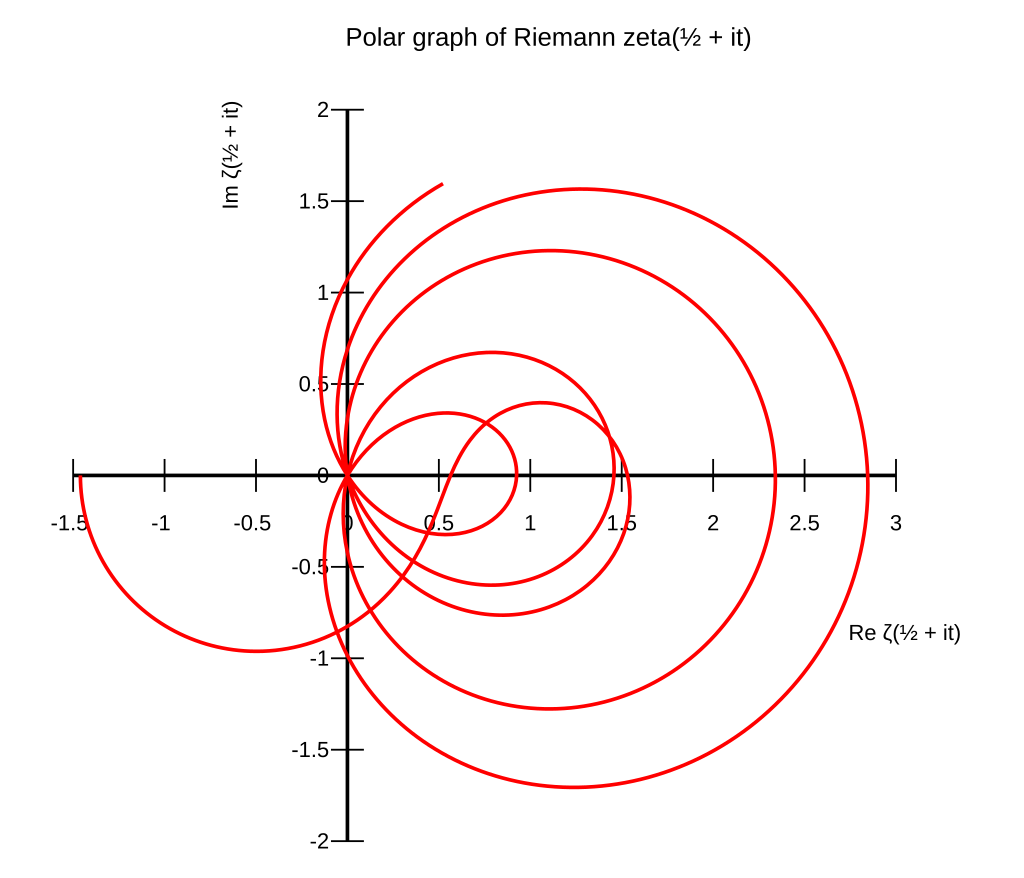
\includegraphics[width=0.6\textwidth]{figure/zeta.png}
    \caption{Referensi Gambar}
    \label{fig:3.ref_gbr}
    {\footnotesize Sumber: internet}
\end{figure}

\subsection{\textit{Teori 2}} \label{II.teori3}
\lipsum[3-4] % Menampilkan paragraf 3 sampai 4 dari lorem ipsum
Berikut adalah ilustrasi konsep yang digunakan seperti pada Gambar \ref{fig:3.ref_gbr2}. \par
\begin{figure}[H] % Posisi gambar tepat dibawah teks
  \centering
  
\includegraphics[width=0.7\textwidth]{figure/Logo_ITERA.png}
  \caption{Ilustrasi Konsep}
  \label{fig:3.ref_gbr2}
  {\footnotesize Sumber: dokumentasi penelitian}
\end{figure}

\subsection{Metrik Performa: MAE, RMSE} \label{II.mae}
\textit{Mean Absolute Error} (MAE) \cite{Suryanto2019MAE} \cite{cort2005maermse}. Rumus perhitungan dari MAE dapat dilihat pada \ref{eq:2.mae}. \par

\begin{equationcaptioned}[eq:2.mae]{
    MAE = \frac{1}{n} \sum_{i=1}^{n} \left| y_i - \hat{y}_i \right|
}{
    Mean Absolute Error (MAE)
}
\end{equationcaptioned}
    \newpage
\chapter{METODE PENELITIAN} \label{Bab III}

\section{Alur Penelitian} \label{III.Alur}
Pada penelitian ini, alur dirancang untuk memastikan setiap tahapan pemrosesan dilakukan secara sistematis dan efisien. Alur penelitian ini mencerminkan langkah-langkah utama yang dilakukan pada penelitian ini, dapat dilihat pada Gambar \ref{fig:3.alur}. \par

\begin{figure}[H] % Kalau menggunakan H, posisi gambar akan tepat dibawah teks
    \centering
    
\includegraphics[width=0.8\textwidth]{figure/samplephoto.jpg}
    \caption{Alur Penelitian}
    \label{fig:3.alur}
\end{figure}

\section{Penjabaran Langkah Penelitian} \label{III.Jabar Alur}
Untuk memperjelas setiap langkah-langkah yang telah didefinisikan pada Gambar \ref{fig:3.alur}, berikut ini akan dijelaskan secara rinci tahapan-tahapan yang dilakukan dalam penelitian ini.

\subsection{Identifikasi Masalah} \label{III.Identifikasi_masalah}
\lipsum[1] % Menampilkan paragraf 1 sampai 2 dari lorem ipsum


\section{Alat dan Bahan Tugas Akhir} \label{III.Alat dan Bahan}
Dalam menjalani penelitian, beberapa alat dan bahan digunakan untuk memastikan penelitian berjalan dengan baik.\par

\subsection{Alat} \label{III.Alat}
Dalam membuat pengukuran frekuensi denyut nadi non-kontak dalam penelitian, berikut adalah alat-alat yang digunakan: \par
\begin{enumerate}[noitemsep]
	\item \textit{Visual Studio Code} sebagai \textit{tools} untuk \textit{text editor}.
	\item Python versi 3.12.5
        \item OpenCV versi 4.10.0.84
	\item NumPy versi 2.1.1
	\item Mediapipe versi 0.10.14
	\item Scipy versi 1.12.0
        \item Matplotlib versi 3.8.3
        \item Flask versi 3.1.0
\end{enumerate}

\subsection{Bahan} \label{III.Bahan}
Dataset yang digunakan pada penelitian ini merupakan dataset 

\section{Ilustrasi Perhitungan Metode} \label{III.Ilustrasi}
Dalam penelitian ini, hasil perhitungan dari program akan melalui serangkaian pengujian untuk mengevaluasi tingkat keakuratan model yang digunakan. Data dummy tersebut dapat dilihat pada Tabel \ref{table:3.dummy}. \par

\begin{longtable}{|c|>{\centering\arraybackslash}p{1.1cm}|>{\centering\arraybackslash}p{1.1cm}|>{\centering\arraybackslash}p{1.1cm}|>{\centering\arraybackslash}p{1.1cm}|>{\centering\arraybackslash}p{1.1cm}|>{\centering\arraybackslash}p{1.1cm}|>{\centering\arraybackslash}p{1.1cm}|>{\centering\arraybackslash}p{1.1cm}|}
	\caption{Data \textit{dummy} Pengujian}
	\label{table:3.dummy}\\
	\hline
	\multirow{2}{*}{\textbf{Subjek}} & \multicolumn{7}{|c|}{\textbf{Hasil Prediksi (BPM)}} & \multirow{2}{*}{\textbf{GT}} \\ \cline{2-8}
    & \textbf{F} & \textbf{NA} & \textbf{NO} & \textbf{RC} & \textbf{LC} & \textbf{M} & \textbf{C} & \\ 
        \hline
	   \endfirsthead
       \hline
       \multirow{2}{*}{\textbf{Subjek}} & \multicolumn{7}{|c|}{\textbf{Hasil Prediksi (BPM)}} & \multirow{2}{*}{\textbf{GT}} \\ \cline{2-8}
    & \textbf{F} & \textbf{NA} & \textbf{NO} & \textbf{RC} & \textbf{LC} & \textbf{M} & \textbf{C} & \\ 
    \hline
	\endhead
	\hline
	\endfoot
	\hline
	\endlastfoot
	1 & 68 & 69 & 68 & 70 & 68 & 71 & 69 & 68 \\ 
	\hline
	2 & 69 & 69 & 68 & 70 & 68 & 71 & 69 & 69 \\
	\hline
	3 & 70 & 70 & 69 & 71 & 68 & 73 & 69 & 70\\
	\hline
	4 & 71 & 70 & 70 & 72 & 69 & 73 & 70 & 71 \\
	\hline
	5 & 72 & 72 & 70 & 72 & 70 & 74 & 70 & 72 \\
	\hline
        6 & 73 & 72 & 71 & 74 & 71 & 76 & 71 & 73 \\ 
	\hline
	7 & 74 & 73 & 72 & 74 & 72 & 77 & 71 & 74 \\
	\hline
	8 & 75 & 74 & 72 & 74 & 73 & 77 & 73 & 75\\
	\hline
	9 & 76 & 75 & 73 & 75 & 74 & 78 & 75 & 76 \\
	\hline
	10 & 77 & 76 & 74 & 78 & 75 & 78 & 76 & 77
\end{longtable}
    \newpage
\chapter{HASIL DAN PEMBAHASAN} \label{Bab IV}

\section{Penggunaan Dataset} \label{IV.Penggunaan}
Dataset yang digunakan pada penelitian ini merupakan dataset PURE. 
\lipsum[1-2] % Menampilkan paragraf 1 sampai 2 dari lorem ipsum


\section{Akuisisi Gambar} \label{IV.Akuisisi}
Pada tahap ini, proses pembacaan dataset dilakukan dengan seksama untuk memastikan setiap gambar diperoleh dengan urutan yang benar dan sistematis. Penting untuk memastikan bahwa gambar yang diperoleh terurut dalam format \textit{time-series} agar memudahkan analisis pergerakan wajah yang terjadi dalam video. Implementasi kode yang digunakan untuk proses ini dapat dilihat pada \cref{code:4.akuisisi}. \par

\begin{lstlisting}[caption={Akuisisi Gambar}, label={code:4.akuisisi}, basicstyle=\ttfamily\scriptsize]
DATASET_ROOT = os.path.join(os.getcwd(), 'PURE Dataset')
def get_all_dataset_folders(root_path):
    dataset_folders = []
    for root, dirs, files in os.walk(root_path):
        if any(file.endswith('.png') for file in files):
            dataset_folders.append(root)
    return dataset_folder
def process_dataset(dataset_path):
    image_files = glob(os.path.join(dataset_path, '*.png'))
    image_files.sort()
    for image_file in image_files:
        frame = cv2.imread(image_file)
        if frame is None:
            continue
        frame_rgb = cv2.cvtColor(frame, cv2.COLOR_BGR2RGB)
        cv2.imshow('Frame', frame)
        if cv2.waitKey(1) & 0xFF == ord('q'):
            break
    cv2.destroyAllWindows()
def main():
    datasets = get_all_dataset_folders(DATASET_ROOT)
    for dataset in datasets:
        process_dataset(dataset)
\end{lstlisting}


\cref{code:4.akuisisi} merupakan baris kode untuk melakukan akuisisi gambar. 


\section{Analisis Hasil Penelitian} \label{IV.Analisis}
\lipsum[1-2] % Menampilkan paragraf 1 sampai 2 dari lorem ipsum


\section{Pembahasan} \label{IV.Bahas}
\lipsum[1-2] % Menampilkan paragraf 1 sampai 2 dari lorem ipsum
    \newpage
\chapter{KESIMPULAN DAN SARAN} \label{Bab V}

\section{Kesimpulan} \label{V.Kesimpulan}
Berdasarkan penelitian yang telah dilakukan, maka kesimpulan yang diperoleh adalah sebagai berikut:
\begin{enumerate}
    \item Berdasarkan pengujian 
    \item mengimplementasikan
\end{enumerate}

\section{Saran} \label{V.Saran}
Adapun saran yang dapat diberikan untuk penelitian lebih lanjut berdasarkan penelitian ini adalah sebagai berikut:\par
\begin{enumerate}
    \item Pengembangan 
    \item Tampilan 
\end{enumerate}
    %----------------------------------------------------------------%

    % Daftar Pustaka
    \newpage
    \phantomsection% 
    \addcontentsline{toc}{chapter}{DAFTAR PUSTAKA}
    \printbibliography[title={Daftar Pustaka}]

    % Lampiran
    % TODO: Tabel Lampiran
    \newpage
    \appendix
    \addcontentsline{toc}{chapter}{LAMPIRAN}
    \chapter*{Lampiran}
    \renewcommand\thesection{\Alph{section}}
    \input{chapters/appendix}

\end{document}
